\documentclass[a4paper]{article}

\usepackage[T2A]{fontenc}
\usepackage[utf8]{inputenc}
\usepackage[russian]{babel}


\usepackage{graphicx}
\usepackage{float}
\usepackage{mathtools}
\usepackage{wrapfig}
\usepackage{amsfonts, amssymb, amsmath, latexsym}
\usepackage{nicefrac}
\usepackage{hhline}
\usepackage{multirow}
\usepackage[colorinlistoftodos,bordercolor=orange,backgroundcolor=orange!20,linecolor=orange,textsize=scriptsize]{todonotes}
\usepackage[colorlinks=true,linkcolor=blue,citecolor=blue]{hyperref}       % hyperlinks
\usepackage{nicefrac}       % compact symbols for 1/2, etc.
\usepackage{nameref}
\usepackage{booktabs}       % professional-quality tables

\usepackage{algorithm}
\usepackage{algpseudocode}

\usepackage{xcolor, colortbl}
\usepackage{etoolbox}

% \graphicspath{ {./} }

\usepackage[verbose=true,letterpaper]{geometry}

\newgeometry{
    textheight=9in,
    textwidth=5.5in,
    top=1in,
    headheight=12pt,
    headsep=25pt,
    footskip=30pt
}

\usepackage{epigraph}

%

\newcommand{\argmin}{\mathop{\arg\!\min}}
\newcommand{\argmax}{\mathop{\arg\!\max}}

\newcommand{\Var}{\mathbb{V}}
\newcommand{\Exp}{\mathbb{E}}
\newcommand{\Cov}{\text{Cov}}
\newcommand{\makebold}[1]{\boldsymbol{#1}}
\newcommand{\mean}[1]{\overline{#1}}
\newcommand{\eps}{\varepsilon}
\renewcommand{\epsilon}{\varepsilon}

\newcommand{\partfrac}[2]{\frac{\partial #1}{\partial #2}}
\newcommand{\ttt}[1]{\texttt{#1}}
\newcommand{\term}[1]{\textbf{#1}}

\newcommand{\la}{\langle}
\newcommand{\ra}{\rangle}

\newcommand{\lp}{\left(}
\newcommand{\rp}{\right)}
\newcommand{\lf}{\left\{}
\newcommand{\rf}{\right\}}
\newcommand{\ls}{\left[}
\newcommand{\rs}{\right]}
\newcommand{\lv}{\left|}
\newcommand{\rv}{\right|}

\newcommand*{\affaddr}[1]{#1} % No op here. Customize it for different styles.
\newcommand*{\affmark}[1][*]{\textsuperscript{#1}}


\usepackage{amsthm}

\theoremstyle{definition}
\newtheorem{definition}{Определение}[section]

\newtheorem{exercise}{Задача}[section]

\newtheorem*{solution}{Решение}
\theoremstyle{remark}
\newtheorem*{remark}{Remark}

\makeatletter
\renewcommand{\l@section}{\@dottedtocline{1}{0em}{2.1em}}
\makeatother

% \setlength\epigraphwidth{.8\textwidth}
\setlength\epigraphrule{0pt}

\title{Работа 3.5.1 \\ Изучение плазмы газового разряда в неоне}
\author{Шарапов Денис, Зелёный Николай, Б05-005}
\date{}

\usepackage{fancyhdr}
\pagestyle{fancy}
\fancyhf{}
\rhead{Работа 3.5.1}
\lhead{}
\cfoot{\thepage}
\usepackage{subcaption}
\usepackage[font={small}]{caption}

\begin{document}

    \maketitle
    \tableofcontents
    \newpage
    
\section{Аннотация}

 \textbf{Цель работы:} изучить вольт-амперную характеристику тлеющего разряда и свойства плазмы методом зондовых характеристик.\\
 
 \noindent \textbf{В работе используются:} стеклянная газоразрядная трубка, наполненная неоном, высоковольтный источник питания, источник питания постоянного тока, делитель напряжения, резистор, потенциометр, ампермометры, вольтметры, переключатели.
 
 \section{Теоретические сведения}
 
 \subsection{Плазма}

В ионизированном газе поле ионов <<экранируется>> электронами. Для поля $\mathbf{E}$ и плотности $\rho$ электрического заряда

$$\text{div}~\mathbf{E} = 4 \pi \rho, $$

а с учётом сферической симметрии и $\mathbf{E} = -\text{grad}~\varphi$:

\begin{equation}
    \dfrac{d^2 \varphi}{dr^2}+\dfrac{2}{r}\dfrac{d\varphi}{dr}=-4\pi \rho.
\end{equation}

\begin{wrapfigure}{r}{100pt}
    \centering
    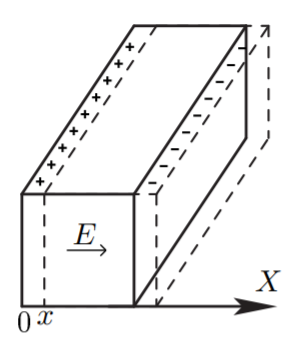
\includegraphics[width = 100pt]{image/first.png}
\end{wrapfigure} 

Плотности заряда электронов и ионов (которые мы считаем бесконечно тяжёлыми и поэтому неподвижными)

\begin{equation}
\begin{array}{c}
    \rho_e = -ne \cdot \exp\left(\dfrac{e\varphi}{kT_e}\right),\\
    \rho_i = ne.
\end{array}
\end{equation}

Тогда из $(1)$ в предположении $\dfrac{e\varphi}{kT_e} \ll 1$ получим

\begin{equation}
    \varphi = \dfrac{Ze}{r}e^{-r/r_D},
\end{equation}

где $r_D = \sqrt{\dfrac{kT_e}{4\pi n e^2}}$ -- \textit{радиус Дебая}. Среднее число ионов в сфере такого радиуса 
  

\begin{equation}
    N_D = n\dfrac{4}{3}\pi r_D^2.
\end{equation}

Теперь выделим параллелепипед с плотностью $n$ электронов, сместим их на $x$. Возникнут поверхностные заряды $\sigma = nex$, поле от которых будет придавать электронам ускорение:
$$
\dfrac{d^2x}{dt^2}=-\dfrac{eE}{m}=-\dfrac{4\pi n e^2}{m}x.
$$ 
Отсюда получаем \textit{плазменную (ленгмюровскую) частоту} колебаний электронов:
\begin{equation}
\omega_p = \sqrt{\dfrac{4\pi ne^2}{m}}.
\end{equation}
 
\subsection{Одиночный зонд}

При внесении в плазму уединённого проводника -- \textit{зонда} с потенциалом, изначально равным потенциалу точки плазмы, в которую его помещают, на него поступают токи электроннов и ионов:

\begin{equation}
\begin{array}{c}
I_{e0} = \dfrac{n \langle v_e \rangle}{4}eS,\\
I_{i0} = \dfrac{n \langle v_i \rangle}{4}eS,
\end{array}
\end{equation}

\begin{wrapfigure}{r}{120pt}
    \centering
    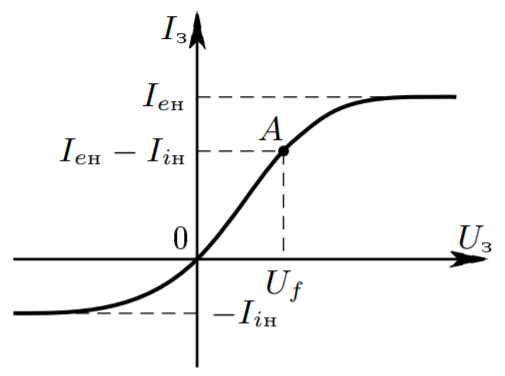
\includegraphics[width = 120pt]{image/second.png}
\end{wrapfigure} 

где $\langle v_e \rangle$ и $\langle v_i \rangle$ --- средние скорости электронов и ионов, $S$ --- площадь зонда, $n$ --- плотность электронов и ионов. Скорости электронов много больше скорости ионов, поэтому $I_{i0} \ll I_{e0}$. Зонд будет заряжаться до некоторого равновестного напряжения $U_f$~--- \textit{плавающего потенциала}.\\

В равновесии ионный ток мало меняется, а электронный имеет вид

$$ I_e = I_0 \exp\left( -\dfrac{eU_f}{kT_e} \right). $$

Будем подавать потенциал $U_\text{з}$ на зонд и снимать значение зондового тока $I_\text{з}$. Максимальное значение тока $I_{e\text{н}}$ -- электронный ток насыщения, а минимальное $I_{i\text{н}}$ -- ионный ток насыщения. Значение из эмпирической формулы Бомона:

\begin{equation}
    I_{i\text{н}} = 0.4 neS \sqrt{\dfrac{2kT_e}{m_i}}.
\end{equation}

\subsection{Двойной зонд}

Двойной зонд -- система из двух одинаковых зондов, расположенных на небольшом расстоянии друг от друга, между которыми создаётся разность потенциалов, меньшая $U_f$. Рассчитаем ток между ними вблизи $I=0$. При небольших разностях потенциалов ионные токи на оба зонда близки к току насыщения и компенсируют друг друга, а значит величина результирующего тока полностью связана с разностью электронных токов. Пусть потенциалы на зондах

$$U_1 = -U_f + \Delta U_1, $$
$$ U_2 = -U_f + \Delta U_2. $$

Между зондами $U = U_2 - U_1 = \Delta U_2 - \Delta U_1$. Через первый электрод

\begin{equation}
    I_1 = I_{i\text{н}} + I_{e1} = I_{i\text{н}} - \dfrac{1}{4}neS\langle v_e\rangle \exp\left(-\dfrac{eU_f}{kT_e}\right)\exp\left(\dfrac{e\Delta U_1}{kT_e}\right)=I_{i\text{н}}\left(1 - \exp\left( \dfrac{e\Delta U_1}{kT_e} \right)\right).
\end{equation}


Аналогично через второй получим

\begin{equation}
    I_2 = I_{i\text{н}}\left(1 - \exp\left( \dfrac{e\Delta U_2}{kT_e} \right)\right).
\end{equation}
  
Из $(7)$ и $(8)$ с учётом последовательного соединение зондов ($I_1 = -I_2 = I)$:
$$\Delta U_1= \dfrac{kT_e}{e}\text{ln}\left(1 - \dfrac{I}{I_{i\text{н}}}\right),$$
$$\Delta U_2= \dfrac{kT_e}{e}\text{ln}\left(1 + \dfrac{I}{I_{i\text{н}}}\right).$$

Тогда итоговые формулы для разности потенциалов и тока

\begin{equation}
    U = \dfrac{kT_e}{e}\text{ln}\dfrac{1 - I/I_{i\text{н}}}{1 + I/I_{i\text{н}}}, 
    I = I_{i\text{н}} \text{th}\dfrac{eU}{2kT_e}.
\end{equation}

\begin{wrapfigure}{r}{120pt}
    \centering
    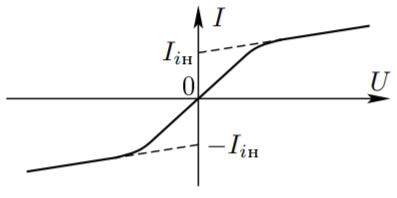
\includegraphics[width = 120pt]{image/third.png}
\end{wrapfigure} 

Реальная зависимость выглядит несколько иначе и описывается формулой 

\begin{equation}
    I = I_{i\text{н}} \text{th}\dfrac{eU}{2kT_e} + AU.
\end{equation}

Из этой формулы можно найти формулу для $T_e$: для $U=0$ мы найдём $I_{i\text{н}}$, продифференцируем в точке $U=0$ и с учётом $\text{th}~\alpha \approx \alpha$ при малых $\alpha$ и $A\rightarrow 0$ получим:

\begin{equation}
    kT_e = \dfrac{1}{2}\dfrac{eI_{i\text{н}}}{\dfrac{dI}{dU}|_{U=0}}.
\end{equation}

\subsection{Установка}

    Стеклянная газоразрядная трубка имеет холодный (ненакаливаемый) полый катод, три анода и \textit{геттерный} узел -- стеклянный баллон, на внутреннюю повехность которого напылена газопоглощающая плёнка (\textit{геттер}). Трубка наполнена изотопом неона $^2_2$Ne при давлении 2 мм рт. ст. Катод и один из анодом (I и II) с помощью переключателя $\Pi_1$ подключается через балластный резистор $R_\text{б}$ ($\approx 450$ кОм) к регулируемому ВИП с выкодным напряжением до 5 кВ.
    При подключении к ВИП анода-I между ним и катодом возникает газовый разряд. Ток разряда измеряется миллиамперметром $A_1$, а падение напряжения на разрядной трубке -- цифровым вольтметром $V_1$, подключённым к трубке черезе высокоомный (25 МОм) делитель напряжения с коэффициентом $(R_1+R_2)/R_2 = 10$.
    При подключении к ВИП анода-II разряд возникает в пространстве между катодом и анодом-II, где находятся двойной зонд, используемый для диагностики плазмы положительного столба. Зонды изготовлены из молибденовой проволоки диаметром $d = 0,2$ мм и имеют длину $l = 5,2$ мм. Они подключены к источнику питания GPS через потенциометр $R$. Переключатель $\Pi_2$ позволяет изменять полярность напряжения на зондах. Величина напряжения на зондах изменяеься с помощью дискретного переключателя <<$V$>> выходного напряжения источника питания и потенциометра $R$, а измеряется цифровым вольтметром $V_2$. Для измерения зондового тока используется мультиметр $A_2$.

    \begin{figure}[h!]
        \centering
        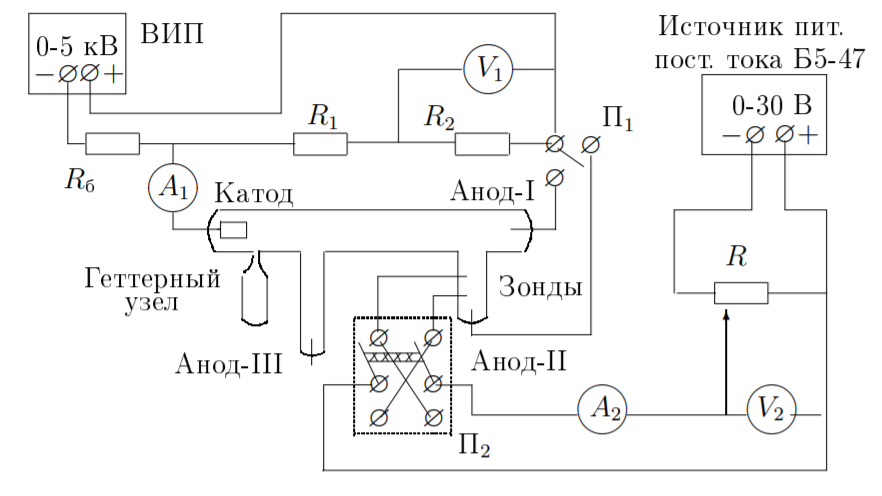
\includegraphics[width = 300pt]{image/scheme.png}
    \end{figure}

\section{Результаты измерений и обработка данных}

\subsection{Вольт-амперная характеристика разряда}

Плавно увеличивая выходное напряжение ВИП, определим напряжение зажигания разряда $U_{\text{заж}} = 30,9 \pm 0,2$ В. \medskip

C помощью вольтметра $V_1$ и амперметра $A_1$ снимем вольт-амперную характеристику (ВАХ) разряда $U_p(I_p)$ (1 дел = 0,04 мА). Результаты измерений представлены в таблице 1.

\begin{table}[h!]
    \centering
    \caption{Результаты измерений для ВАХ}
    \begin{tabular}{|c|c|c|c|}
    \hline
    \multicolumn{2}{|c|}{Возрастание} & \multicolumn{2}{c|}{Убывание} \\ \hline
    $I$, дел         & $U$, В         & $I$, дел       & $U$, В       \\ \hline
    31               & 32,09          & 83             & 27,10        \\ \hline
    36               & 31,76          & 77             & 27,05        \\ \hline
    40               & 31,33          & 69             & 27,00        \\ \hline
    46               & 30,06          & 61             & 28,42        \\ \hline
    50               & 29,64          & 59             & 28,70        \\ \hline
    55               & 29,15          & 54             & 29,21        \\ \hline
    59               & 28,76          & 48             & 29,70        \\ \hline
    65               & 28,25          & 42             & 30,67        \\ \hline
    71               & 27,84          & 36             & 32,07        \\ \hline
    77               & 27,61          & 31             & 32,84        \\ \hline
    84               & 27,33          & 22             & 32,85        \\ \hline
    89               & 27,16          & 16             & 35,04        \\ \hline
    94               & 27,08          & 11             & 65,96        \\ \hline
    \end{tabular}
    \end{table}

    По полученной таблице построим график зависимости $U_p(I_p)$ (погрешности меньше цены деления осей).

    \begin{figure}[h!]
        \centering
        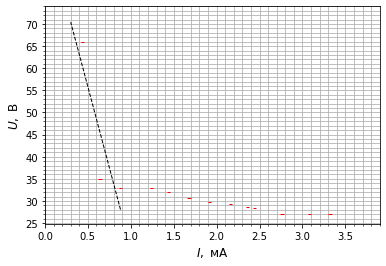
\includegraphics[width = 300pt]{image/graph2.png}
        \caption{График зависимости $U_p(I_p)$}
    \end{figure}

    По наклону прямой определим максимальное дифференциальное сопротивление разряда: $$R_{\text{диф}} = (7,3 \pm 2,1)\cdot 10^4 \; \text{Ом}.$$

    \subsection{Зондовые характеристики}

    Снимем зондовые характеристики при токах разряда, равных 5, 3, 1,5 мА. Результаты измерений запишем в таблицу 3. Получим зависимость $I_{\text{з}}(U_{\text{з}})$.

    \begin{figure}[h!]
        \centering
        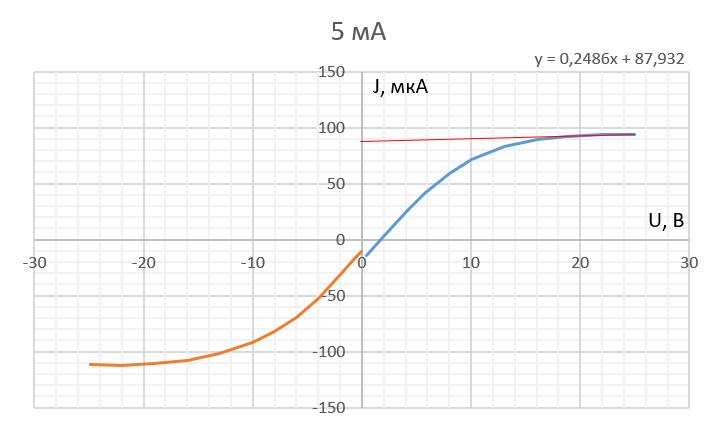
\includegraphics[width = 250pt]{image/graph5.png}
        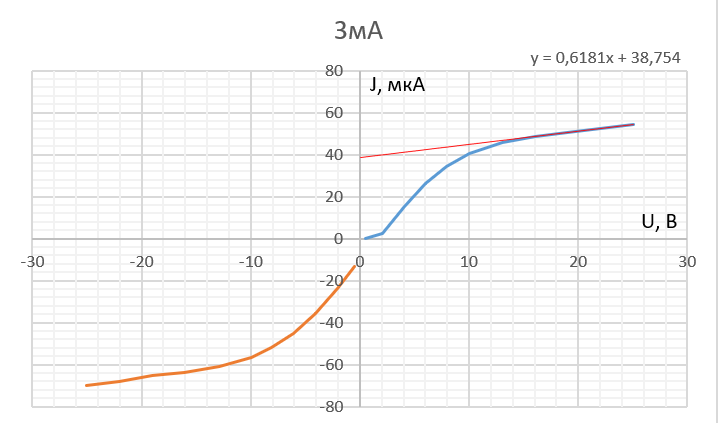
\includegraphics[width = 250pt]{image/graph3.png}
        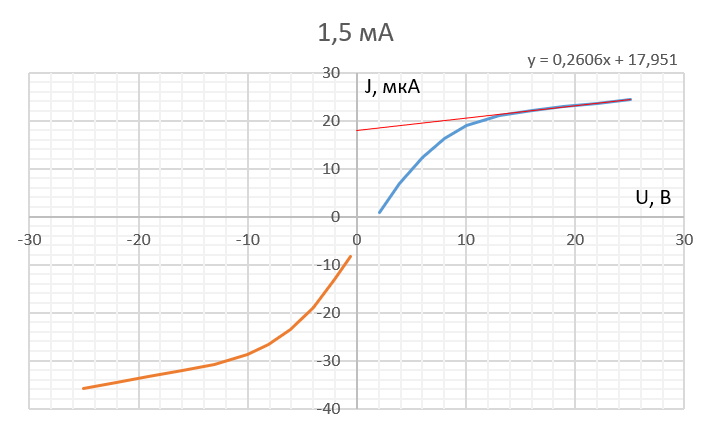
\includegraphics[width = 250pt]{image/graph15.png}
        \caption{Графики зависимости $I_{\text{з}}(U_{\text{з}})$ при различных $I_p$}
    \end{figure}

    Используя данные из таблицы 3, получим величины, определяемые формулами (3), (4), (5), (7), и (12). Результаты внесём в таблицу 2.

        \begin{table}[h!]
            \centering
            \caption{Результаты измерения величин}
            \begin{tabular}{|c|c|c|c|c|c|}
            \hline
            \multicolumn{1}{|l|}{$J_{\text{iн}}$, мкА} & $T\cdot 10^3$, K & $n \cdot 10^13$, м$^{-3}$ & $\omega \cdot 10^4$, рад/с & $r_{D_{e}}\cdot 10^{-2}$, cм & $r_{D} \cdot 10^{-3}$, см \\ \hline
            $87,60 \pm 1,10$                           & $50,4 \pm 5,0$   & $67,9 \pm 8,0$            & $1,45 \pm 0,10$            & $4,35 \pm 0,3$               & 5,64                      \\ \hline
            $38,80 \pm 0,04$                           & $22,4 \pm 3,0$   & $45,0 \pm 5,0$            & $1,18 \pm 0,08$            & $5,35 \pm 0,5$               & 4,62                      \\ \hline
            $18,00 \pm 0,10$                           & $10,3 \pm 3,0$   & $30 \pm 4,0$              & $0,56 \pm 0,04$            & $6,55 \pm 0,8$               & 8,49                      \\ \hline
            \end{tabular}
            \end{table}

            \newpage

            \begin{table}[t!]
                \centering
                \caption*{Таблица 2: Продолжение}
                \begin{tabular}{|c|c|}
                \hline
                $N \cdot 10^5$ & $\alpha \cdot 10^{-11}$ \\ \hline
                2,34           & 2,52                    \\ \hline
                2,89           & 1,67                    \\ \hline
                3,53           & 1,12                    \\ \hline
                \end{tabular}
                \end{table}

            По таблице 2 построим график зависимости $n_e(I_p)$.

            \begin{figure}[h!]
                \centering
                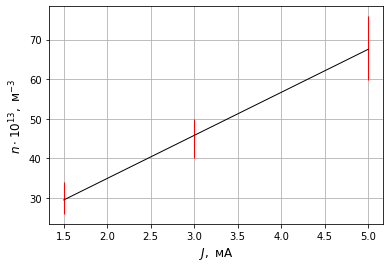
\includegraphics[width = 260pt]{image/graphlast.png}
                \caption{График зависимости $U_p(I_p)$}
            \end{figure}

    \begin{table}[h!]
        \centering
        \caption{Результаты измерений зависимости $I_{\text{з}}(U_{\text{з}})$}
        \begin{tabular}{|c|c|c|c|c|c|}
        \hline
        \multicolumn{2}{|c|}{1,5 мА} & \multicolumn{2}{c|}{3 мА} & \multicolumn{2}{c|}{5 мА} \\ \hline
        $U$, В       & $I$, мкА      & $U$, В      & $I$, мкА    & $U$, В      & $I$, мкА    \\ \hline
        25,067       & 24,5          & 25,11       & 54,28       & 25          & 94          \\ \hline
        22,064       & 23,67         & 22,046      & 52,37       & 22,07       & 93,7        \\ \hline
        18,93        & 22,9          & 19,043      & 50,53       & 18,83       & 92,48       \\ \hline
        16,097       & 22,15         & 16,064      & 48,67       & 16,096      & 89,48       \\ \hline
        13,035       & 21,15         & 13,069      & 45,97       & 13,065      & 83          \\ \hline
        10,005       & 18,95         & 10,041      & 40,72       & 10,022      & 71,27       \\ \hline
        8,039        & 16,31         & 7,922       & 34,24       & 8,02        & 59,45       \\ \hline
        6            & 12,22         & 6,048       & 26,17       & 5,697       & 41,16       \\ \hline
        3,94         & 6,83          & 4,07        & 15,37       & 4,15        & 26,35       \\ \hline
        2,07         & 0,8           & 2,05        & 2,3         & 2,03        & 3,56        \\ \hline
        -25          & -35,9         & 0,54        & -0,08       & 0,46        & -14,48      \\ \hline
        -22          & -34,66        & -25         & -70,23      & -24,9       & -111,4      \\ \hline
        -19,044      & -33,41        & -22         & -68         & -22,055     & -112,4      \\ \hline
        -16,019      & -32,13        & -19         & -65         & -18,994     & -111,05     \\ \hline
        -13,081      & -30,79        & -16,086     & -63,6       & -16         & -108        \\ \hline
        -10,007      & -28,74        & -12,9       & -60,98      & -13,022     & -102,11     \\ \hline
        -8,07        & -26,66        & -9,9        & -56,5       & -10,007     & -92,14      \\ \hline
        -6,074       & -23,55        & -8,052      & -52         & -8,041      & -82,5       \\ \hline
        -4,005       & -18,94        & -6,085      & -45,22      & -6,017      & -69,2       \\ \hline
        -2,03        & -13,21        & -4,03       & -35,65      & -3,99       & -52,2       \\ \hline
        -0,56        & -8,23         & -2,02       & -23,67      & -2,01       & -32,48      \\ \hline
        \end{tabular}
        \end{table}

\section{Вывод}

        В ходе работы была изучена вольт-амперная характеристика тлеющего разряда, были изучены свойства плазмы методом зондовых характеристик. \medskip

        При изучении ВАХ были определены напрежение зажигания в лампе и максимальное дифференциальное сопротивление заряда. \medskip

        При изучении зондовых характеристик были получены три графика зависимости $I_{\text{з}}(U_{\text{з}})$ при различных $I_p$ (5, 3, 1,5 мА). С их помощью были получены значения величины $I_{\text{iн}} = J_{\text{iн}}$. \medskip

\end{document}
